%! suppress = NonMatchingIf

This section describes the \hardwareversion\ Cow Pi development board, describes the theory of operation for its components, and summarizes the features of its display module.

\subsection{Cow Pi Development Board}

The Cow Pi development board consists of a microcontroller board (\mcuboard), a display module (\displaymoduledescription), a $4 \times 4$ matrix keypad, two momentary buttons, two toggleable switches, and two LEDs.
The board is assembled on a \construction; see Figure~\ref{fig:photograph}.

%! suppress = FileNotFound
\begin{figure}
    \centering
    \includegraphics[scale=0.75]{\photograph}
    \caption{A \hardwareversion\ Cow Pi development board.}\label{fig:photograph}
\end{figure}

The toggleable switches are referred to as the \textbf{left switch} and the \textbf{right switch}, and each can be positioned in the left or right position.
When a switch is in the right position, its logic value is high, by way of a pull-up resistor.
When a switch is in the left position, the switch is grounded, and its logic value is low.

The momentary buttons are referred to as the \textbf{left button} and the \textbf{right button}, and each can be pressed (alternatively, in the down position) or unpressed (alternatively, in the up position).
The buttons are normally-open, and so when a button is unpressed, its logic value is high, by way of a pull-up resistor.
When a button is pressed, the button is grounded, and its logic value is low.

The LEDs are referred to as the \textbf{left LED} and the \textbf{right LED}.
\ifboolexpe{bool{nano-form-factor}}{
    The \textbf{left LED} is aliased to the \mcuboard's built-in LED, and some documents may refer to it as the Cow Pi's \textbf{internal LED}.
    \ifdefstring{\construction}{solderless breadboard}{
        Indeed, Arduino-based mark~1 Cow Pis simply use the \mcuboard's built-in LED as the \textbf{left LED} to reduce clutter on the solderless breadboard.
    }{}
    \ifboolexpe{bool{spi}}{
        Note that the \textbf{left LED} may be of limited use in the Cow Pi \cowpiversion\ due to the \mcuboard's \texttt{D13} pin being used for both the \textbf{left} (built-in) \textbf{LED} and also as for the \texttt{SCK} SPI clock signal.
    }{}
    Some documents may refer to the \textbf{right LED} as the Cow Pi's \textbf{external LED}.
}{}
An LED will illuminate when the corresponding microcontroller output is high, and it will deluminate when the corresponding microcontroller output is low.

The matrix keypad is designed to be scanned using the conventional approach of selectively setting the rows' logic values and reading the columns' resulting logic values.
\ifdefstring{\construction}{solderless breadboard}{Note that mark~1 Cow Pis' keypads cannot be accurately scanned if more than one key is pressed at the same time.
    Further, \textbf{there are no current-limiting protections} (other than the microcontroller's fuses) in place to prevent over-current if simultaneously pressing two keys in the same column shorts a logic-high row to a logic-low row.}{}

The microcontroller communicates with the \displaymoduledescription display module using the
\ifboolexpe{bool{spi}}{Serial Peripheral Interface (SPI) protocol.}{}
\ifboolexpe{bool{i2c}}{Inter-Integrated Circuit (I$^2$C or IIC) protocol, also known as the Two-Wire Interface (TWI) protocol.}{}

\ifboolexpe{bool{spi}}{\ifboolexpe{bool{i2c}}{Figures~\ref{fig:pinouts-nano-spi} and~\ref{fig:pinouts-nano-i2c} show}{Figure~\ref{fig:pinouts-nano-spi} shows}}{\ifboolexpe{bool{i2c}}{Figure~\ref{fig:pinouts-nano-i2c} shows}{}}
which input or output is connected to each of the \mcuboard's pins, as well as which general-purpose input/output register bit corresponds to each pin.

\ifboolexpe{bool{spi}}{
    \begin{figure}
        \centering
        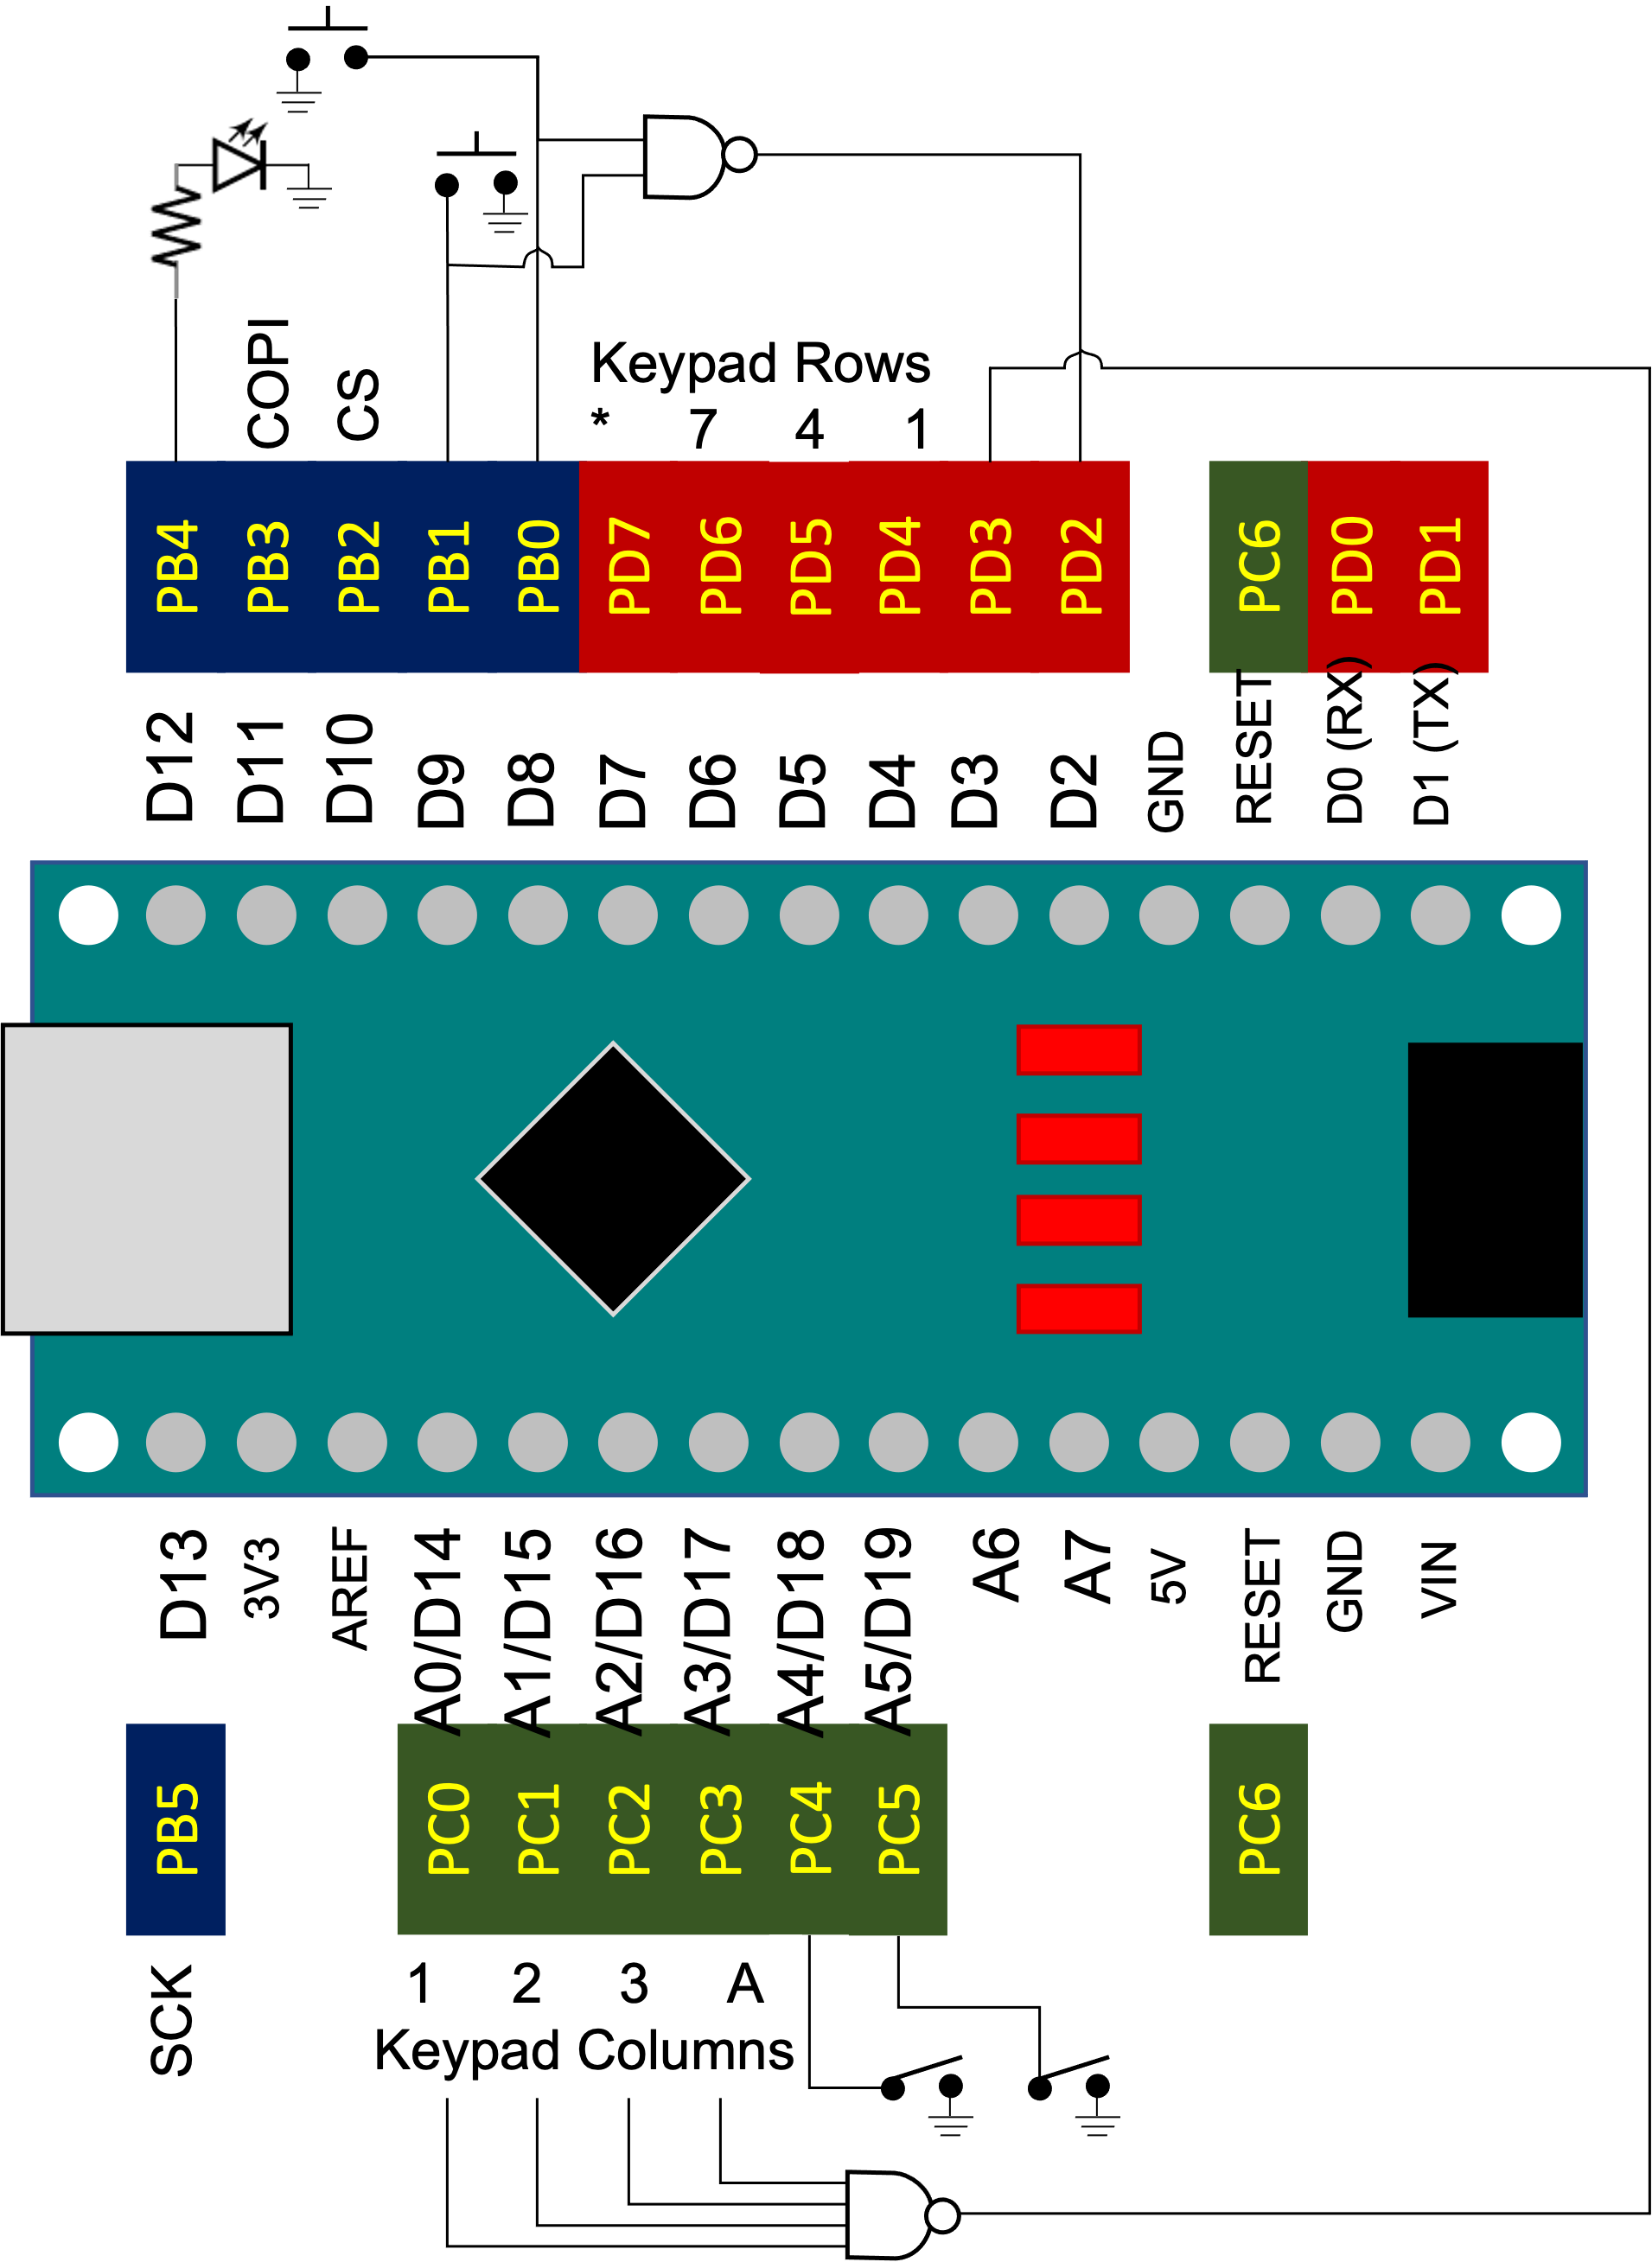
\includegraphics[scale=0.75]{pinouts/nano-spi}
        \caption{Pinout for the \hardwareversion\ Cow Pi development board using \mcuboard and the SPI serial communication protocol.}\label{fig:pinouts-nano-spi}
    \end{figure}
}{}

\ifboolexpe{bool{i2c}}{
    \begin{figure}
        \centering
        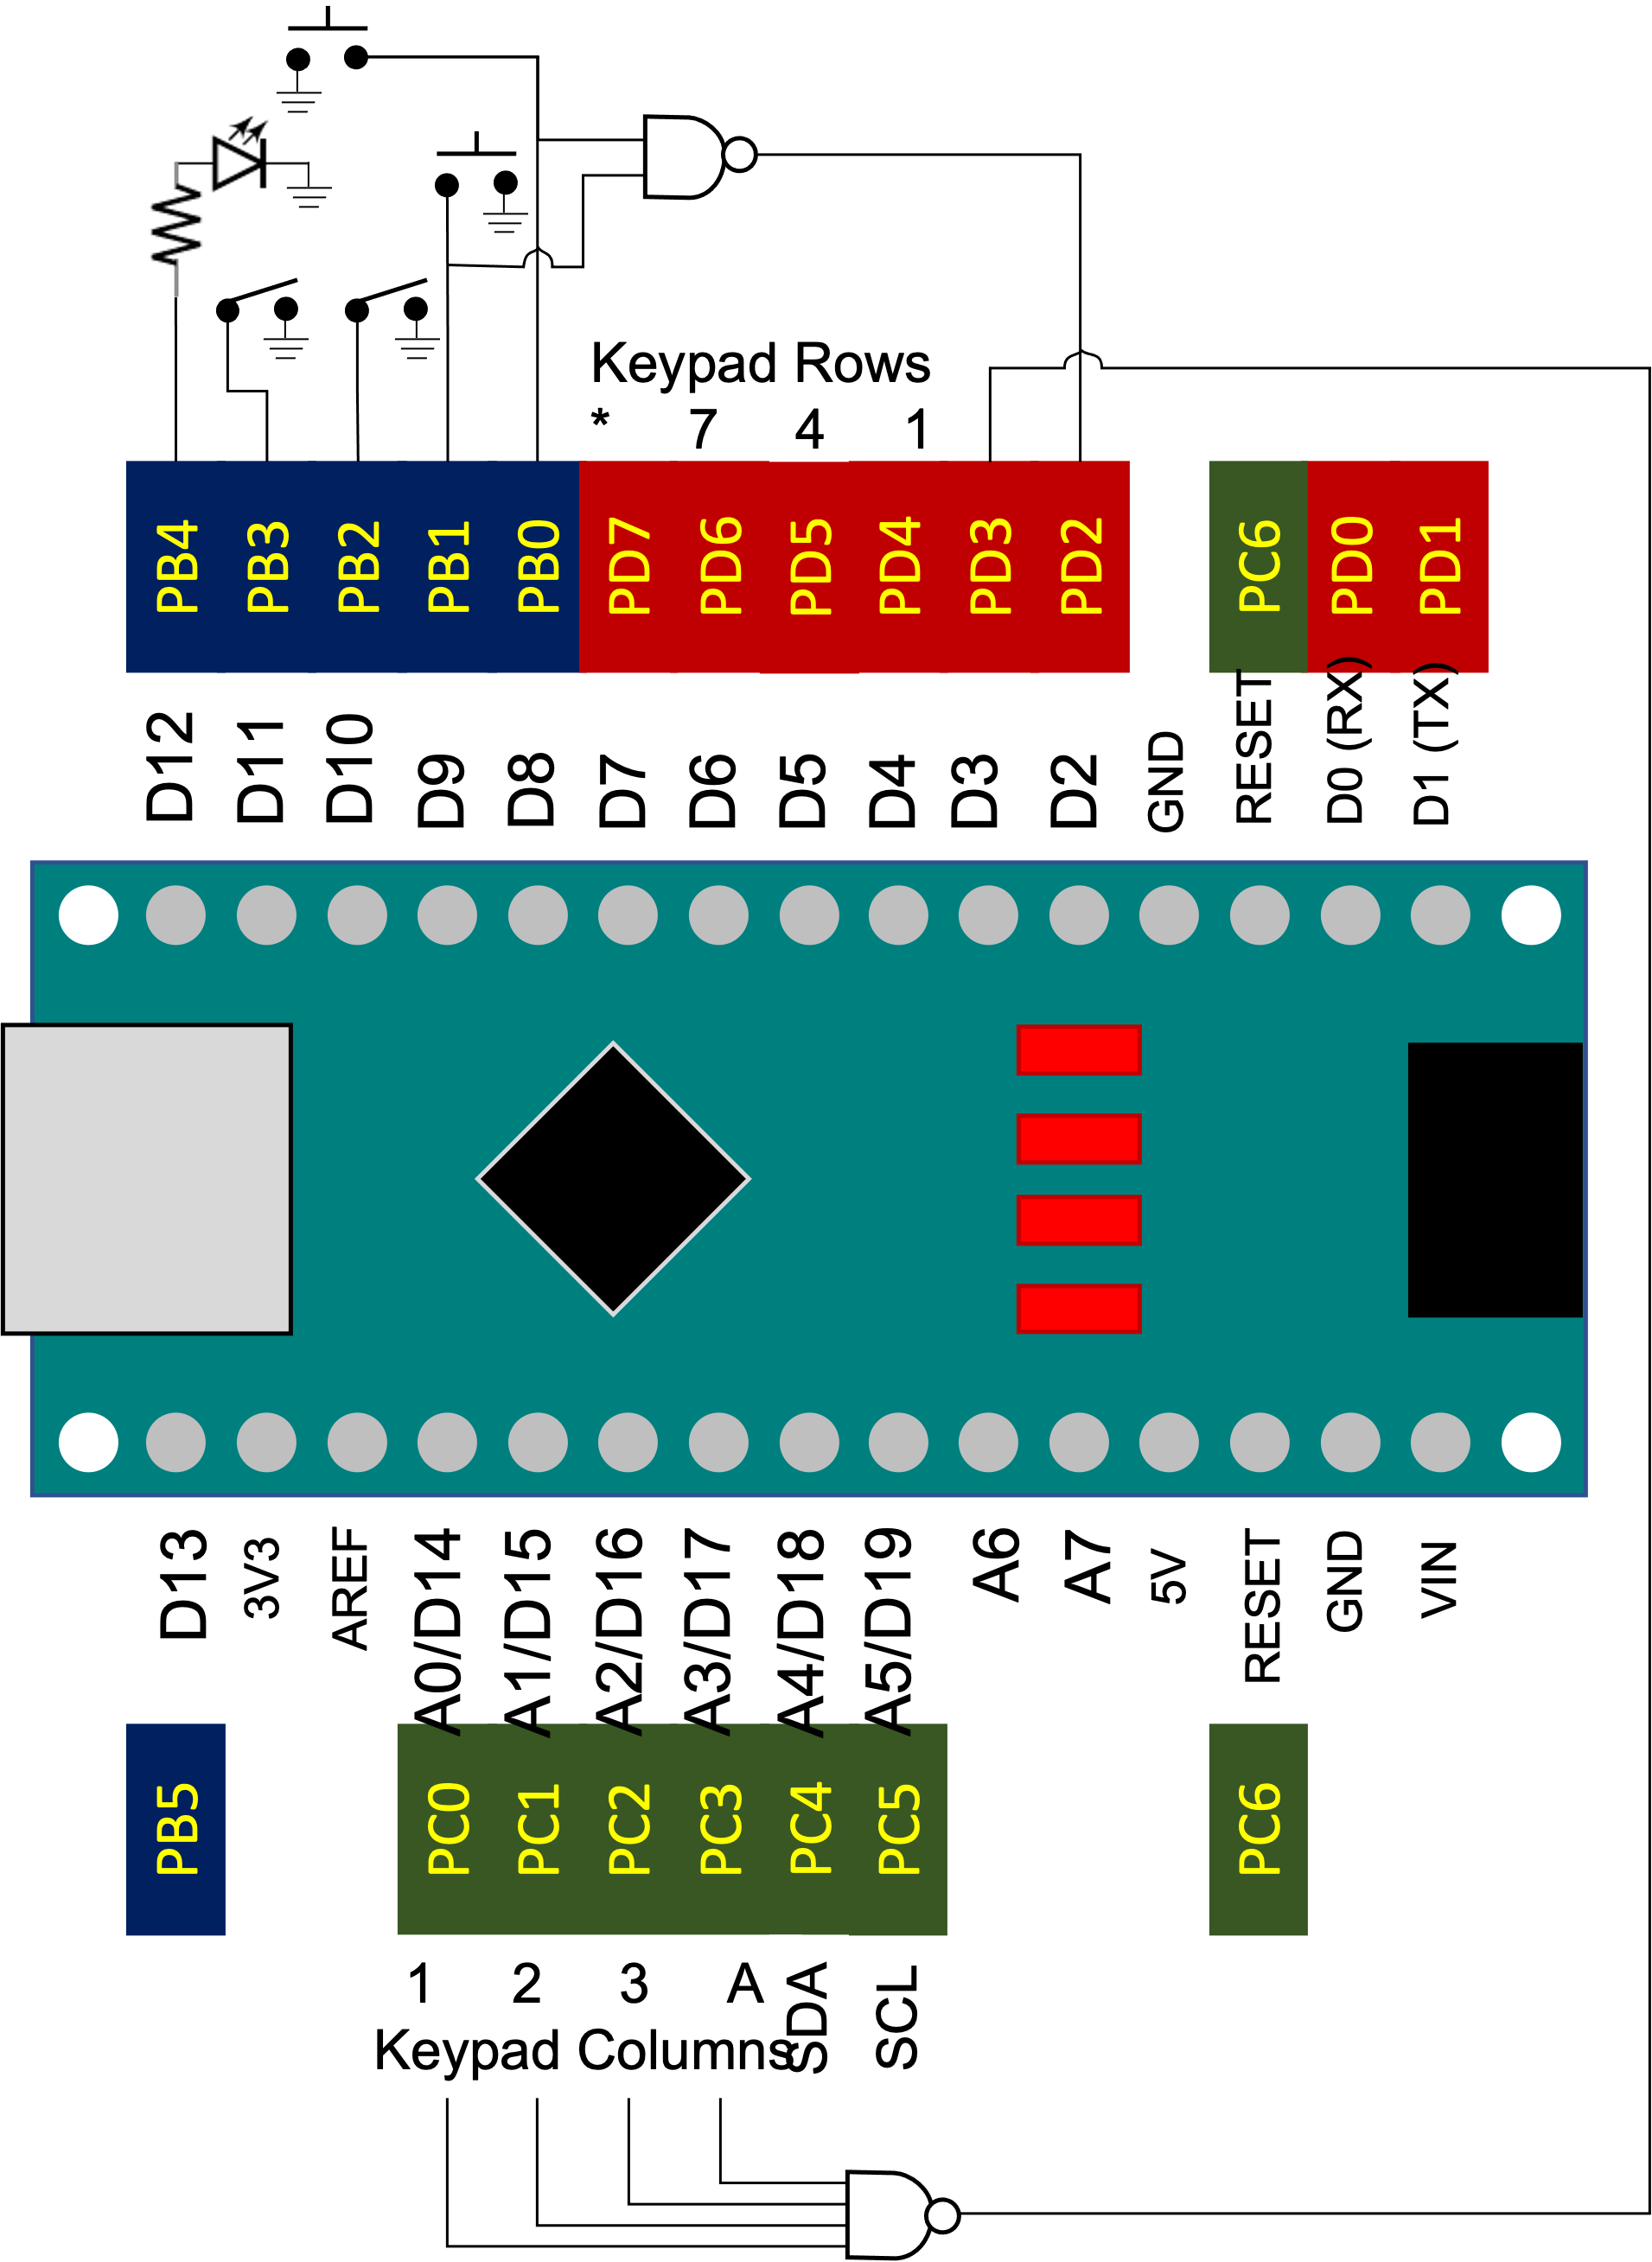
\includegraphics[scale=0.75]{pinouts/nano-i2c}
        \caption{Pinout for a Cow Pi development board using the \mcuboard and the I$^2$C serial communication protocol.}\label{fig:pinouts-nano-i2c}
    \end{figure}
}{}

\subsection{Microcontroller Board}

\subsection{LEDs}

\subsection{Buttons and Switches}

\subsection{Matrix Keypad}

\subsection{Display Module}
